\documentclass{article}
% generated by Madoko, version 1.0.3
%mdk-data-line={1}


\usepackage[heading-base={2},section-num={False},bib-label={True}]{madoko2}


\begin{document}



\mdxtitleblockstart{}
\mdxtitle{纠删码九问}%mdk
\mdxauthorstart{}
\mdxauthorname{360基础架构组王文铎}%mdk
\mdxauthorend\mdtitleauthorrunning{}{}\mdxtitleblockend%mdk

\section{1.\hspace*{0.5em}本文缘起}\label{section}%mdk%mdk

\noindent近期发现很多人都对纠删码很感兴趣,正好我做过纠删码相关的调研工作,因此写了这篇文章。%mdk

本文的部分图片参考了James.Plank教授\href{http://web.eecs.utk.edu/~plank/plank/papers/FAST-2013-Tutorial.html}{一篇很好的综述ppt}.%mdk

\section{2.\hspace*{0.5em}纠删码的背景}\label{section}%mdk%mdk

\subsection{2.1.\hspace*{0.5em}什么是纠删码?为什么叫纠删码?}\label{section}%mdk%mdk

\noindent纠删码起源于通信领域。通信中,我们需要把一大块数据切成很多数据帧来逐次传输。这些帧在传输的过程中可能会出现错误或者干脆整帧被丢掉。
为了解决这一问题,可以将k个原始数据帧编码成n(n\textgreater{}k)个带冗余的新数据帧再进行传输。目的节点接收到足够多的数据帧后,解码得到原始的k个数据帧。%mdk

\textquotedblleft{}编码后某些帧出错了也能解码出原始数据帧\textquotedblright{}的编码叫做纠错码。
\textquotedblleft{}编码后某些帧丢掉了也能解码出原始数据帧\textquotedblright{}的编码叫做纠删码。两者的不同在于,纠错码不知道是否发生了错误及错误的位置,而纠删码明确的知道我们丢失了哪些数据帧。
虽然纠错码更厉害一些,但比如网络的延时/丢包,硬盘损毁等问题,其实是纠删的问题,通过纠删码就可以得到解决。%mdk

\subsection{2.2.\hspace*{0.5em}他们常说mds编码,感觉很厉害,什么叫mds纠删码?}\label{sec-mdsmds}%mdk%mdk

\noindent mds码全名是maxinum distance code. mds码是“编码后的n个数据帧只要还剩余下k个,就能够恢复出原始的k个数据帧”的编码。%mdk

具体的解释:假设我们把k位的二进制数据编码成n位的二进制数据。这个编码C实际上把所有k位二进制数组成的集合$\Omega_k$映射到了所有n位二进制数组成的空间$\Omega_n$.
为了能够解码,这个编码需要是一个单射.意味着映射之后,$\Omega_n$空间中有对应的$2^k$个数据点,设为点集A。%mdk

不妨设A中点a1,a2的汉明距离为A中最小,设为d。即a1,a2有d位是不同的,且A中其他点间至少有d位不同。又不妨设a1,a2来自于$\Omega_k$中的两个点k1,k2。
删除掉a1.a2这d位之后,显然我们没办法去区分a1和a2,也就没办法去区分k1及k2了.%mdk

所以如果设编码的纠删能力为$\theta$,即编码后任意$\theta$位数据丢失,仍能解码出原始的k位数据,有:%mdk
\label{}%mdk
\noindent\mdmathtag{(1)}
\noindent\[\theta <= d - 1
\]%mdk
\noindent同时根据d的定义,A中任意两元素间都至少有d位不同。考虑从$\Omega_n$空间到$\Omega_{n-(d-1)}$空间的一个映射f,f将A中元素的前d-1位删掉。那么A中的元素经过f映射后至少还有1位不同。即f也是一个单射。
又因为编码C也是单射,所以存在一个$\Omega_k$到 $\Omega_{n-(d-1)}$的单射。由单射性质,有
\label{}%mdk
\noindent\mdmathtag{(2)}
\noindent\[\lvert \Omega_k \rvert <= \lvert \Omega_{n-(d-1)} \rvert
\]%mdk
\noindent即:
\label{}%mdk
\noindent\mdmathtag{(3)}
\noindent\[2^k <= 2^{n-d+1}
\]%mdk
\noindent结合(1),可以得到:
\label{}%mdk
\noindent\mdmathtag{(4)}
\noindent\[\theta <= n - k 
\]%mdk
\noindent{} 
我们刚才其实直观的解释了这个道理:将k位数据帧编码成n位数据帧(n-k位冗余),纠错能力理论上最高只有n-k。mds码是达到理论上最高纠错能力的码。
这个结论和进制无关,对数据帧也适用。

另外一个线性的纠删码可以用一个$n*k$的生成矩阵来表示。当生成矩阵的任意$k*k$子方阵可逆(等价于任意k行线性无关)时,编码是mds的。
可以参考后文的RS编码进行证明。%mdk

\section{3.\hspace*{0.5em}存储中的纠删码}\label{section}%mdk%mdk

\subsection{3.1.\hspace*{0.5em}存储系统为什么要用纠删码?}\label{section}%mdk%mdk

\noindent我们知道硬盘经常会坏,坏了数据就丢了。软件层面上我们为了解决这个问题,通常是在分布式系统中存放数据的多个副本。如果一个硬盘坏了,上面数据被抹掉,其他硬盘上的副本可以接管服务,同时通过拷贝恢复数据。
ceph等都是默认实际存放3倍的数据。如果我们要存放大量的冷数据,这样做就会有成本的问题。
恰巧纠删码有恢复丢失数据的作用。可以将数据先分成k块,然后纠删编码成n块,存放到n个不同的硬盘上。
硬盘故障时,可以通过其他硬盘上的数据恢复出原始的k块数据。注意这里只存了一个副本,实际存放了n/k 倍的数据。%mdk

\subsection{3.2.\hspace*{0.5em}RS纠删码实栗。}\label{sec-rs}%mdk%mdk

\noindent我们快速复习下raid的知识。%mdk

\begin{itemize}%mdk

\item{}
raid0为了写入速度将数据条带化并行写入多个硬盘。%mdk%mdk

\item{}
为了防止故障,raid4除了几个存放条带化后数据的硬盘外,还做了一个冗余盘存放其异或值,当一个数据盘故障,可以通过冗余与其他数据盘异或恢复。但由于冗余都在一个盘上,写任何数据都要写一次冗余盘,形成瓶颈。%mdk%mdk

\item{}
raid5在raid4基础上做了优化,将冗余块分所有的数据盘上。使得磁盘的负载均衡。%mdk%mdk
%mdk
\end{itemize}%mdk

\noindent纠删编码存储,其实就是将原始数据条带化成k个数据块,将这k组原始数据块。纠删编码后存于n个硬盘中。为了使得读取时不需要进行矩阵计算,
通常让编码后的n个块中有k个数据块和原始数据块一样。如下图。%mdk

\begin{figure}[tbp]%mdk
\begin{mdcenter}%mdk

\noindent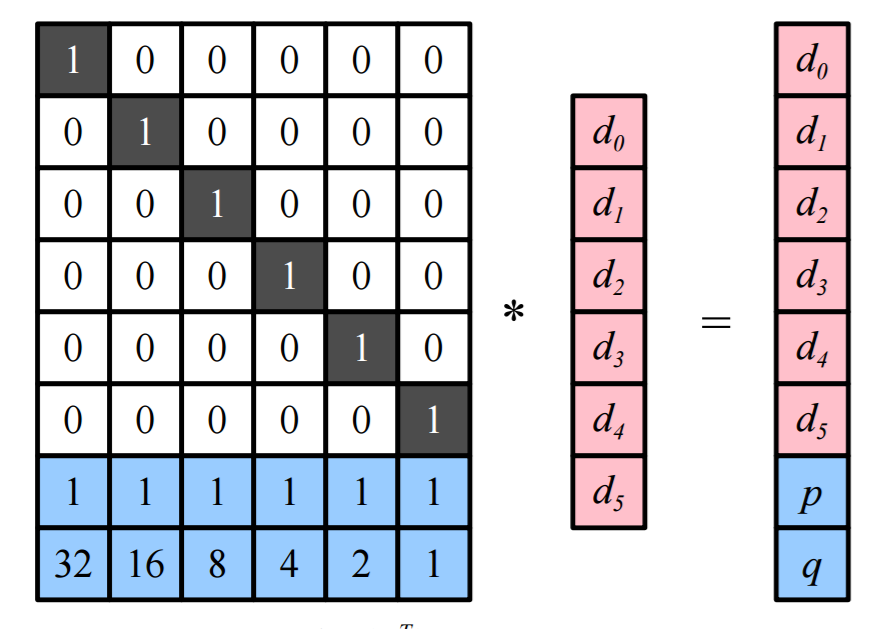
\includegraphics[keepaspectratio=true,width=\dimmin{}{\dimwidth{0.60}}]{images/rs1}{}%mdk

\mdhr{}%mdk

\noindent\mdcaption{\textbf{Figure~\mdcaptionlabel{1}.}~\mdcaptiontext{RS(6,2)}}%mdk
%mdk
\end{mdcenter}%mdk
\end{figure}%mdk

\noindent假设部分硬盘发生了故障,等式右边还剩下至少k个survior,如下图:%mdk

\begin{figure}[tbp]%mdk
\begin{mdcenter}%mdk

\noindent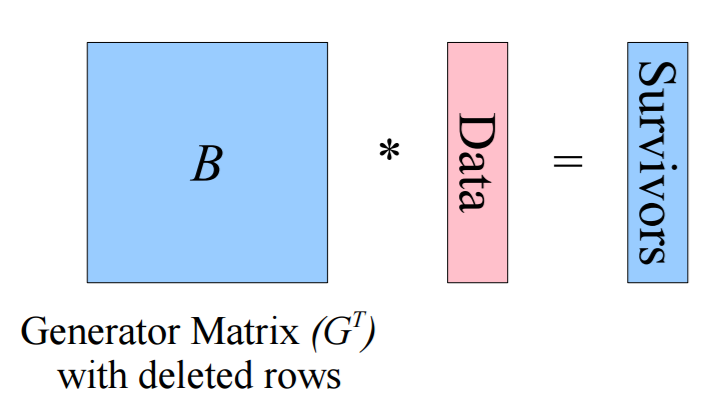
\includegraphics[keepaspectratio=true,width=\dimmin{}{\dimwidth{0.60}}]{images/rs3}{}%mdk

\mdhr{}%mdk

\noindent\mdcaption{\textbf{Figure~\mdcaptionlabel{2}.}~\mdcaptiontext{RS(6,2)}}%mdk
%mdk
\end{mdcenter}%mdk
\end{figure}%mdk

\noindent那么如果B可逆,就有:%mdk

\begin{figure}[tbp]%mdk
\begin{mdcenter}%mdk

\noindent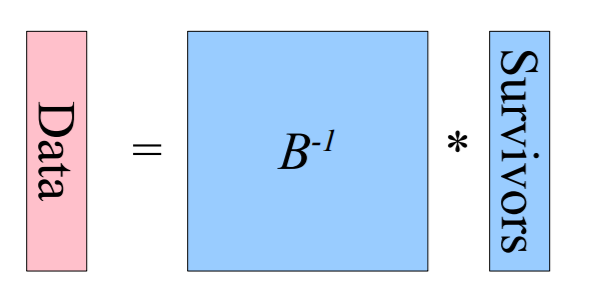
\includegraphics[keepaspectratio=true,width=\dimmin{}{\dimwidth{0.60}}]{images/rs5}{}%mdk

\mdhr{}%mdk

\noindent\mdcaption{\textbf{Figure~\mdcaptionlabel{3}.}~\mdcaptiontext{RS(6,2)}}%mdk
%mdk
\end{mdcenter}%mdk
\end{figure}%mdk

\noindent也即恢复了原始数据。由此我们可以看到,构造一个mds的RS纠删码关键是找个合适的矩阵S.其和I 拼接后的矩阵,任意$k*k$子方阵可逆。
我们熟悉的范德蒙矩阵和柯西矩阵都满足这个性质。 ceph采用的纠删码库 jerasure 就是采用范德蒙矩阵来构造生成矩阵。%mdk

\subsection{3.3.\hspace*{0.5em}LRC纠删}\label{sec-lrc}%mdk%mdk

\subsubsection{3.3.1.\hspace*{0.5em}有了mds的RS纠删码,为什么还要有LRC纠删码?}\label{sec-mdsrslrc}%mdk%mdk

\noindent衡量分布式系统有两个重要指标,可用性和可靠性。可用性指系统平均可以正常工作的时间。而可靠性是指系统在t时间内正常工作的概率。
所以谈可靠性一定要有时间。比如一个系统每1秒内都有1ms不能正常工作,那么他的可用性是99.9\%。而一小时内不出故障的可靠性是0。
当纠删码对应的数据块发生故障之后,我们需要读冗余及其他数据块,计算出坏掉的数据块内的数据并恢复后才能系统回到可用状态。
因此,可用性很大程度上取决于修复所用的时间。绝大部分的故障,其实只有一个硬盘坏掉,在这种情况下,RS编码为了修复这个坏掉的数据块需要读取全部剩余的数据块及至少一个冗余块。这个过程受到cpu和网卡的限制会很慢。
意味着可用性的降低。而LRC编码正是为了解决这个问题。%mdk

\subsubsection{3.3.2.\hspace*{0.5em}LRC纠删是如何做的?}\label{sec-lrc}%mdk%mdk

\noindent LRC全名是local seperabal code。LRC除了global的冗余块之外,还将数据块分组,给每组数据块增加冗余。这样当一个数据块故障,只需要读取组内的数据块及冗余块,大大提高恢复速度。
下面是RS(12,3) 和 LRC(12,2,1)的对比。%mdk

\begin{figure}[tbp]%mdk
\begin{mdcenter}%mdk

\noindent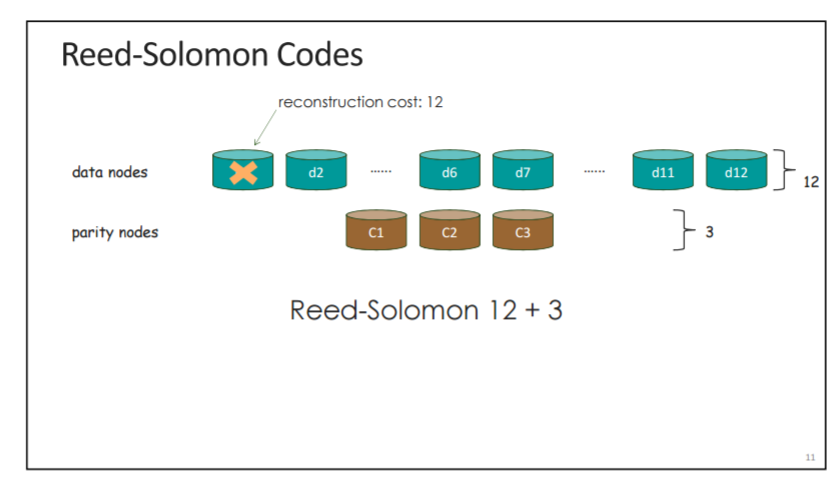
\includegraphics[keepaspectratio=true,width=\dimmin{}{\dimwidth{0.60}}]{images/lrc1}{}%mdk

\mdhr{}%mdk

\noindent\mdcaption{\textbf{Figure~\mdcaptionlabel{4}.}~\mdcaptiontext{RS(12,3)}}%mdk
%mdk
\end{mdcenter}%mdk
\end{figure}%mdk

\begin{figure}[tbp]%mdk
\begin{mdcenter}%mdk

\noindent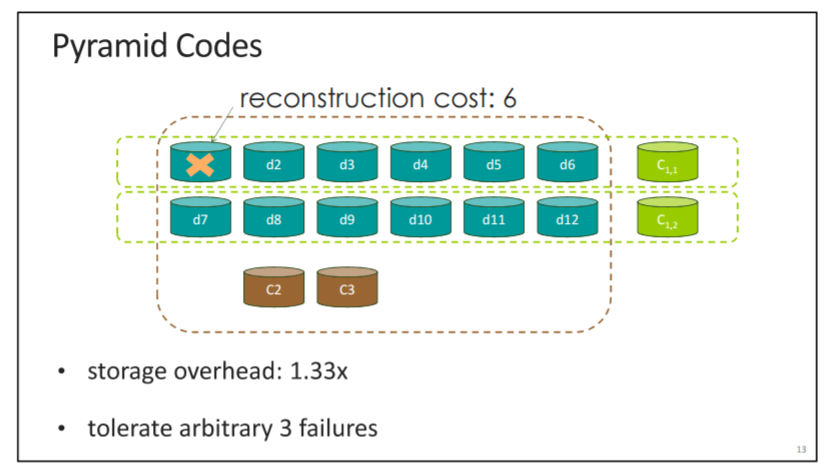
\includegraphics[keepaspectratio=true,width=\dimmin{}{\dimwidth{0.60}}]{images/lrc2}{}%mdk

\mdhr{}%mdk

\noindent\mdcaption{\textbf{Figure~\mdcaptionlabel{5}.}~\mdcaptiontext{LRC(12,2,1)}}%mdk
%mdk
\end{mdcenter}%mdk
\end{figure}%mdk

\noindent由上图可以看到,当一个数据块出现故障,RS(12,3)需要读11个data块加1个冗余块,而LRC(12,2,1)只需要读5个数据块加1个冗余块就可以计算并恢复出故障数据块。
同样能纠删能力下,LRC编码显然会快很多。%mdk

\section{4.\hspace*{0.5em}应用场景}\label{section}%mdk%mdk

\subsection{4.1.\hspace*{0.5em}那么何时应该使用纠删码呢?}\label{section}%mdk%mdk

\noindent根据上面的分析,我们可以看到,如果你的系统使用纠删码而不是主从结构的三副本,这意味着%mdk

\begin{itemize}[noitemsep,topsep=\mdcompacttopsep]%mdk

\item每次写入都要进行矩阵运算并写很多块冗余,延迟高%mdk

\item不管写入还是故障恢复,对cpu和网络的消耗都相对高%mdk

\item纠删码在很少的副本数情况下能够达到3副本同样高的可靠性,存储成本低。%mdk
%mdk
\end{itemize}%mdk

\noindent因此如果cpu,网卡满足要求,纠删码能够很好的降低冷数据的存储成本。%mdk

\subsection{4.2.\hspace*{0.5em}大公司是怎样使用纠删码的?}\label{section}%mdk%mdk

\noindent微软azure 从GFS采用的RS(6,3) 迁移到RS(12,4) 之后又迁移到了LRC(12,2,2).即两个global的冗余块,加每6个数据块对应一个局部冗余块。
而facebook的hdfs 从 RS(10,4) 迁到了 LRC(10,6,5)。%mdk

\subsection{4.3.\hspace*{0.5em}最后的问题,这些纠删码是怎么制定的?}\label{section}%mdk%mdk

\noindent这些公司纠删码肯定是结合线上故障的经验数据加上严密的可靠性计算定出来的。上文的几个纠删码其可靠性都比3副本要高。
可靠性的计算比较复杂,后续也许会写文章来介绍。%mdk%mdk


\end{document}
